\chapter{Data processing with \ctapipe{}}
\label{ch:data-processing}

The analysis in this work was done with the open-access low-level data processing software for \cta{},
\ctapipe{} \cite{ctapipe}. The version used is the development version \texttt{0.15.1.dev166+gf26107f},
henceforth shortened to version \texttt{0.15.1}. The goal of \ctapipe{} is to provide a complete analysis
framework ranging from data calibration and image extraction to the reconstruction of events and the
analysis of their properties. In this chapter, I will describe \ctapipe{} with its different data
levels and the different analysis steps (\autoref{sec:data-levels}). In \autoref{sec:pipeline} I will
explain the full pipeline created for this work.

\section{Data Levels in \ctapipe{}}
\label{sec:data-levels}

There are several data levels in \ctapipe{}, spanning from the raw data \rzero{} to the reconstructed events
\dlt{}, with the raw data levels being denoted by a \textbf{R} and the calibrated data levels by a \textbf{D}.
\autoref{fig:ctapipe} shows a simplified overview of the data levels and the analysis steps.
The raw data level \rzero{} is the data that comes directly from the photodetectors. The time-resolved
signal of the data is calibrated from \rzero{} to \rone{}. Then the data volume gets reduced
(\rone{} \rightarrow \dlz{}) by a selection of waveforms. The \dlz{} data level is the first level being
stored and also the first level to be processed from the simulation datasets used in this work.
From \dlz{} to \dloa{}, the images of the data are extracted from the time pulses, which are then
cleaned by a cleaning algorithm, allowing for parametrization of the events (\dloa{} \rightarrow \dlob{}).
The parametrized events can then be reconstructed (\dlob{} \rightarrow \dlt{}) and stored on the \dlt{} data level.

\begin{figure}
    \centering
    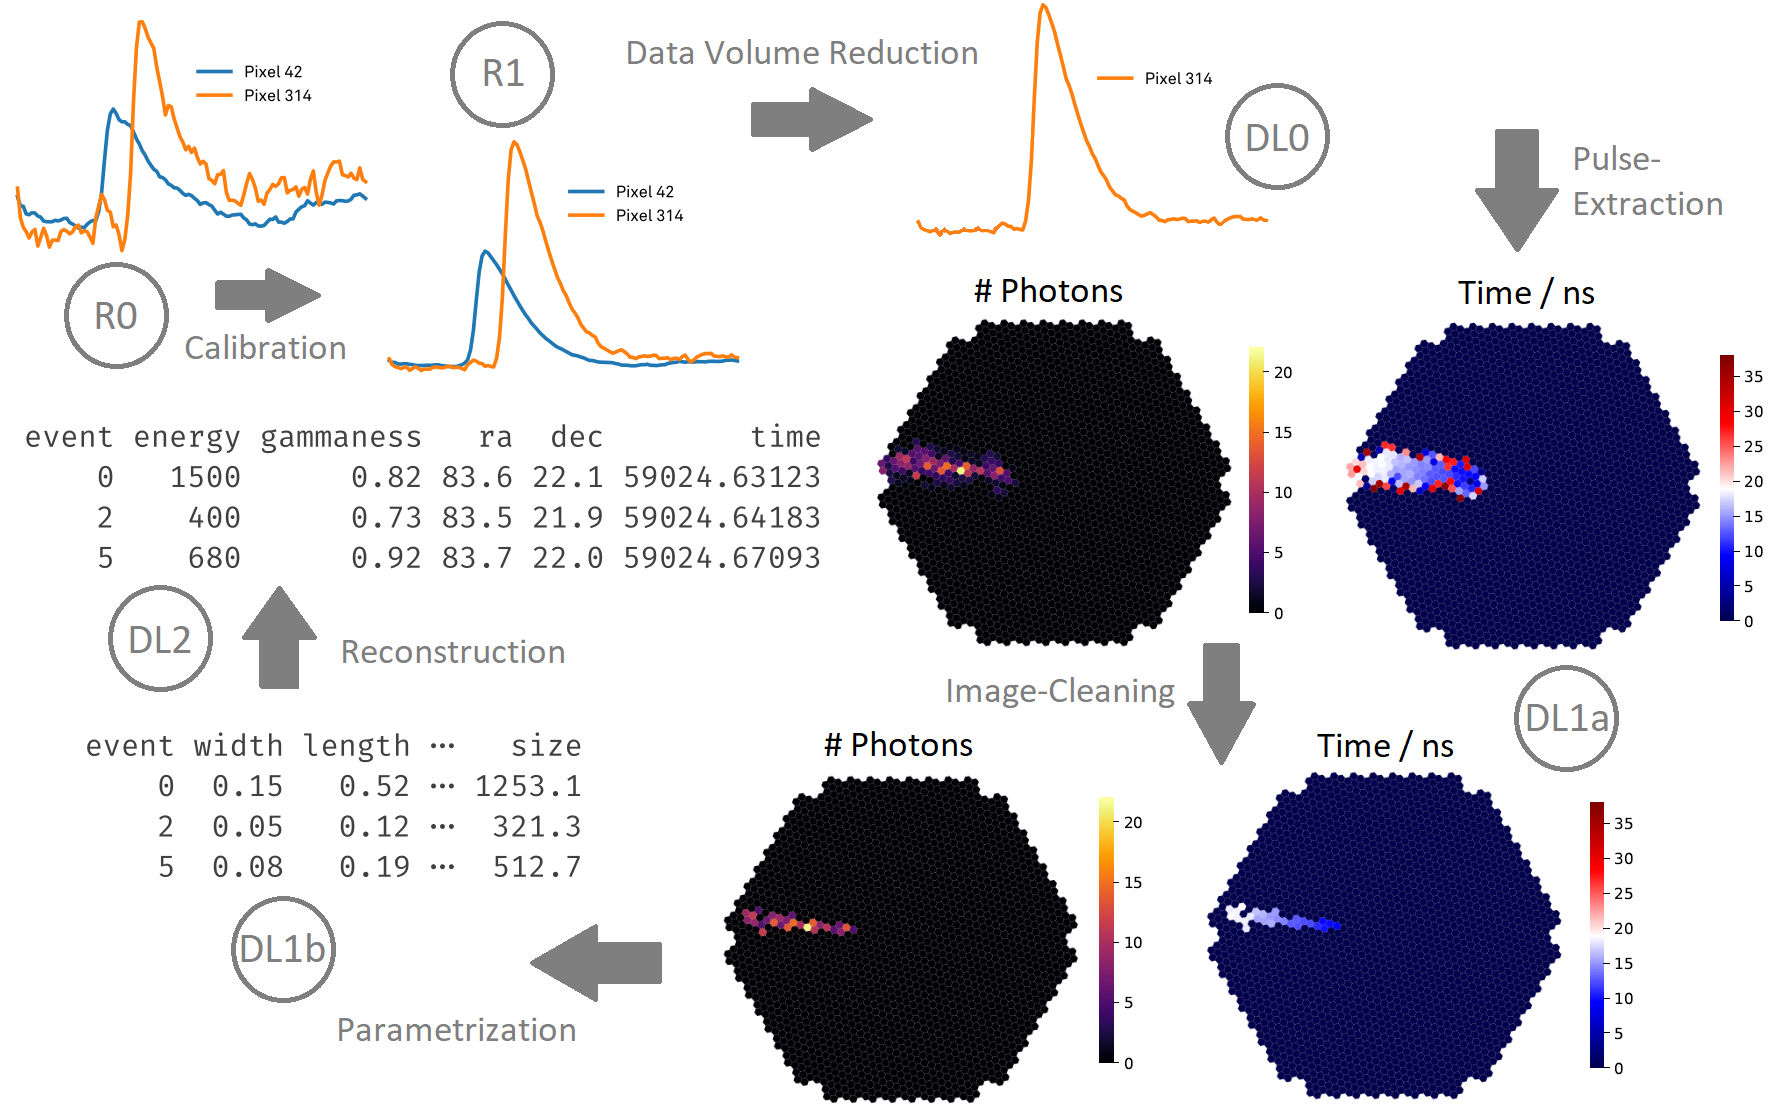
\includegraphics[width=\textwidth]{graphics/ctapipe.png}
    \caption{Data levels in \ctapipe{}. Raw data levels are denoted by a \textbf{R} and calibrated
    data levels by a \textbf{D}. The raw data first gets calibrated (\rzero{} \rightarrow \rone{})
    and then reduced in volume by selecting waveforms (\rone{} \rightarrow \dlz{}). From there the
    images are extracted (\dlz{} \rightarrow \dloa{}) and cleaned with a cleaning algorithm. This
    allows for parametrization of the events (\dloa{} \rightarrow \dlob{}). The parametrized events
    can then be reconstructed (\dlob{} \rightarrow \dlt{}) \cite{noethe_thesis, hackfeld}. \todo[inline]{citation}}
    \label{fig:ctapipe}
\end{figure}

\section{This work's data processing pipeline}
\label{sec:pipeline}

In this work, the data processing pipeline is as follows: First, several simulation data runs are
selected and processed with \ctapipe{}. Then, the datasets are merged and serve as a basis for a re-run
of the combined dataset with various parameter combinations described in \autoref{ch:finding-hyperparams}.
Each resulting dataset can then be processed on an array- or telescope data level, resulting in
\dloa{} image plots, angular resolution and effective area or \todo[color=blue!40]{find alternative wording}efficiency as well as metrics for the
performance. An \todo{wording}in-detail description of how this helps to compare the performance of the different
cleaning algorithms can be found in \autoref{sec:hyperparameters}. \autoref{fig:data-processing} shows
a schematic overview of the data processing pipeline of this work.

\begin{figure}
    \centering
    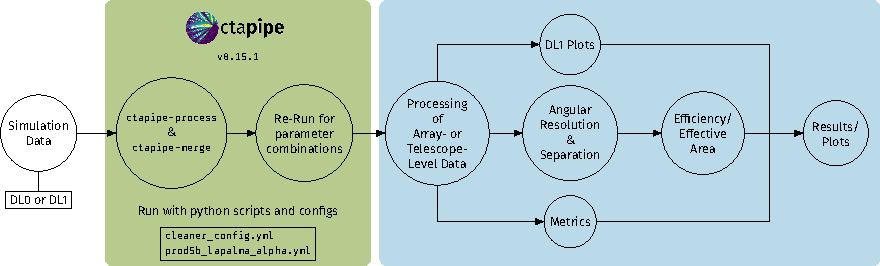
\includegraphics[width=\textwidth]{graphics/data_pipeline.pdf}
    \caption{Schematic overview of the data pipeline used for this work. Single runs of the simulation
    data are processed with \ctapipe\texttt{-process} and then merged via \ctapipe\texttt{-merge}.
    The merged data is then processed on the array- or telescope data level resulting in scores for metrics
    as well as \texttt{dl1 images} and plots for the angular resolution and the effective area.}
    \label{fig:data-processing}
\end{figure}

\todo{think about connections between \autoref{ch:finding-hyperparams} and \autoref{data-processing}}
